\chapter{Transport Injuries}
\label{applications-double_dismod}

A compartmental model is not appropriate for all conditions.  Transport injuries have a wide range of outcomes, ranging from minor scratches to severe brain trauma to death.  Given some suffer acute injury while others sustain chronic conditions, traffic injuries violate the model assumption of a constant mortality hazard.  To address this disparity in mortality risk, transport injuries can be divided into short term and long term outcomes.  This method is also necessary for other injuries and diseases such as heart attack and stroke.

In the GBD 2010 Study, injuries are defined as all conditions codable to the ICD-9 and ICD-10 injuries chapter.  Transport injuries includes all road injuries for pedestrian, bicyclist, motorized two-wheeler rider, occupant in a motorized vehicle with 3 or more wheels, other road-transport injury and unintentional other transport injury.

Data only includes cases warranting hospital care and cases warranting treatment by health care professional but not hospitalization (other health care).  As seen in Figure \ref{fig:app-injury traffic data}, only prevalence and cause-specific mortality were available from verbal autopsy, surveillance systems, surveys, census and police reports.

    \begin{figure}[h]
        \begin{center}
            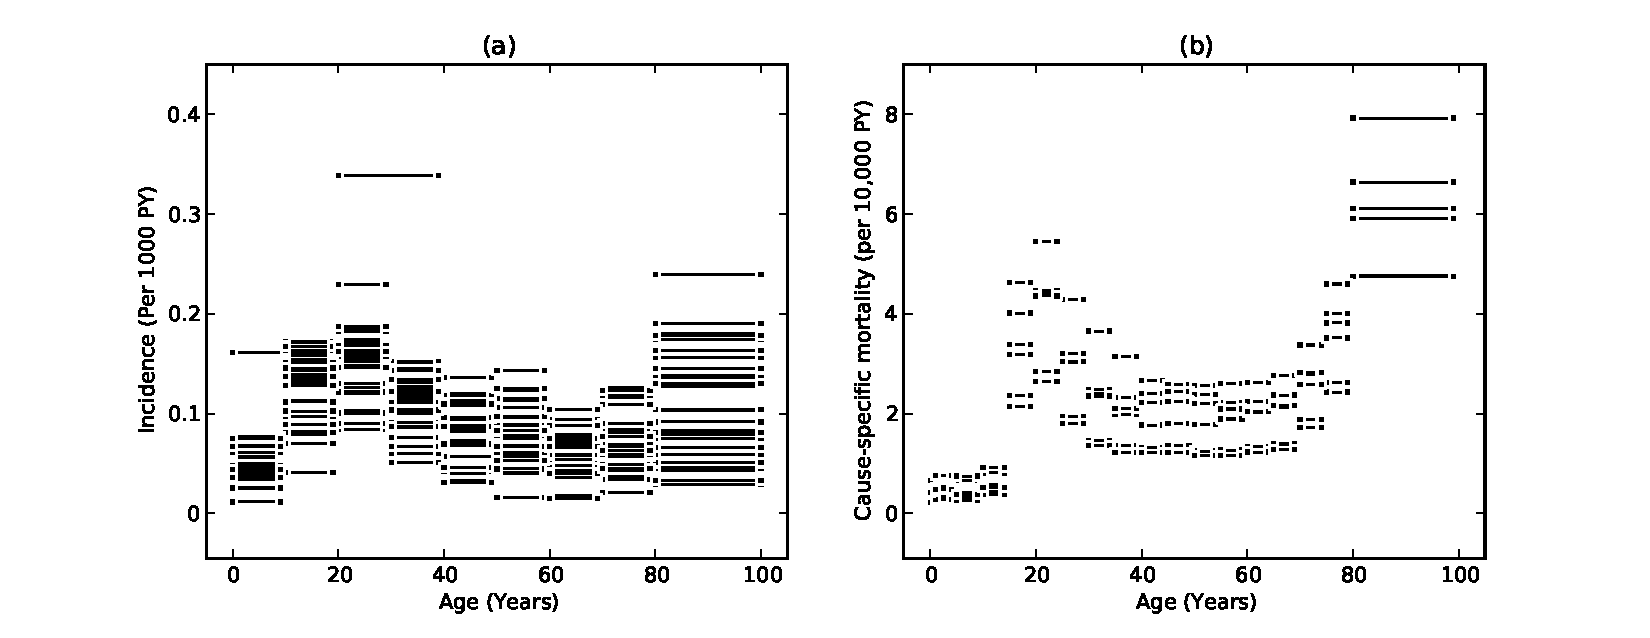
\includegraphics[width=\textwidth]{injury-traffic_data.pdf}
            \caption{Hospital and survey data for road injury and unintentional other transport injury for males in the region of North America, High Income.  Systematic review yielded only incidence (a) and the product of prevalence and excess mortality (b) data.}
            \label{fig:app-injury traffic data}
        \end{center}
    \end{figure}

To make use of both the cause-specific mortality and the prevalence data, a compartmental model first estimates the age-specific burden, as shown in Figure \ref{fig:app-injury traffic fit}

    \begin{figure}[h]
        \begin{center}
            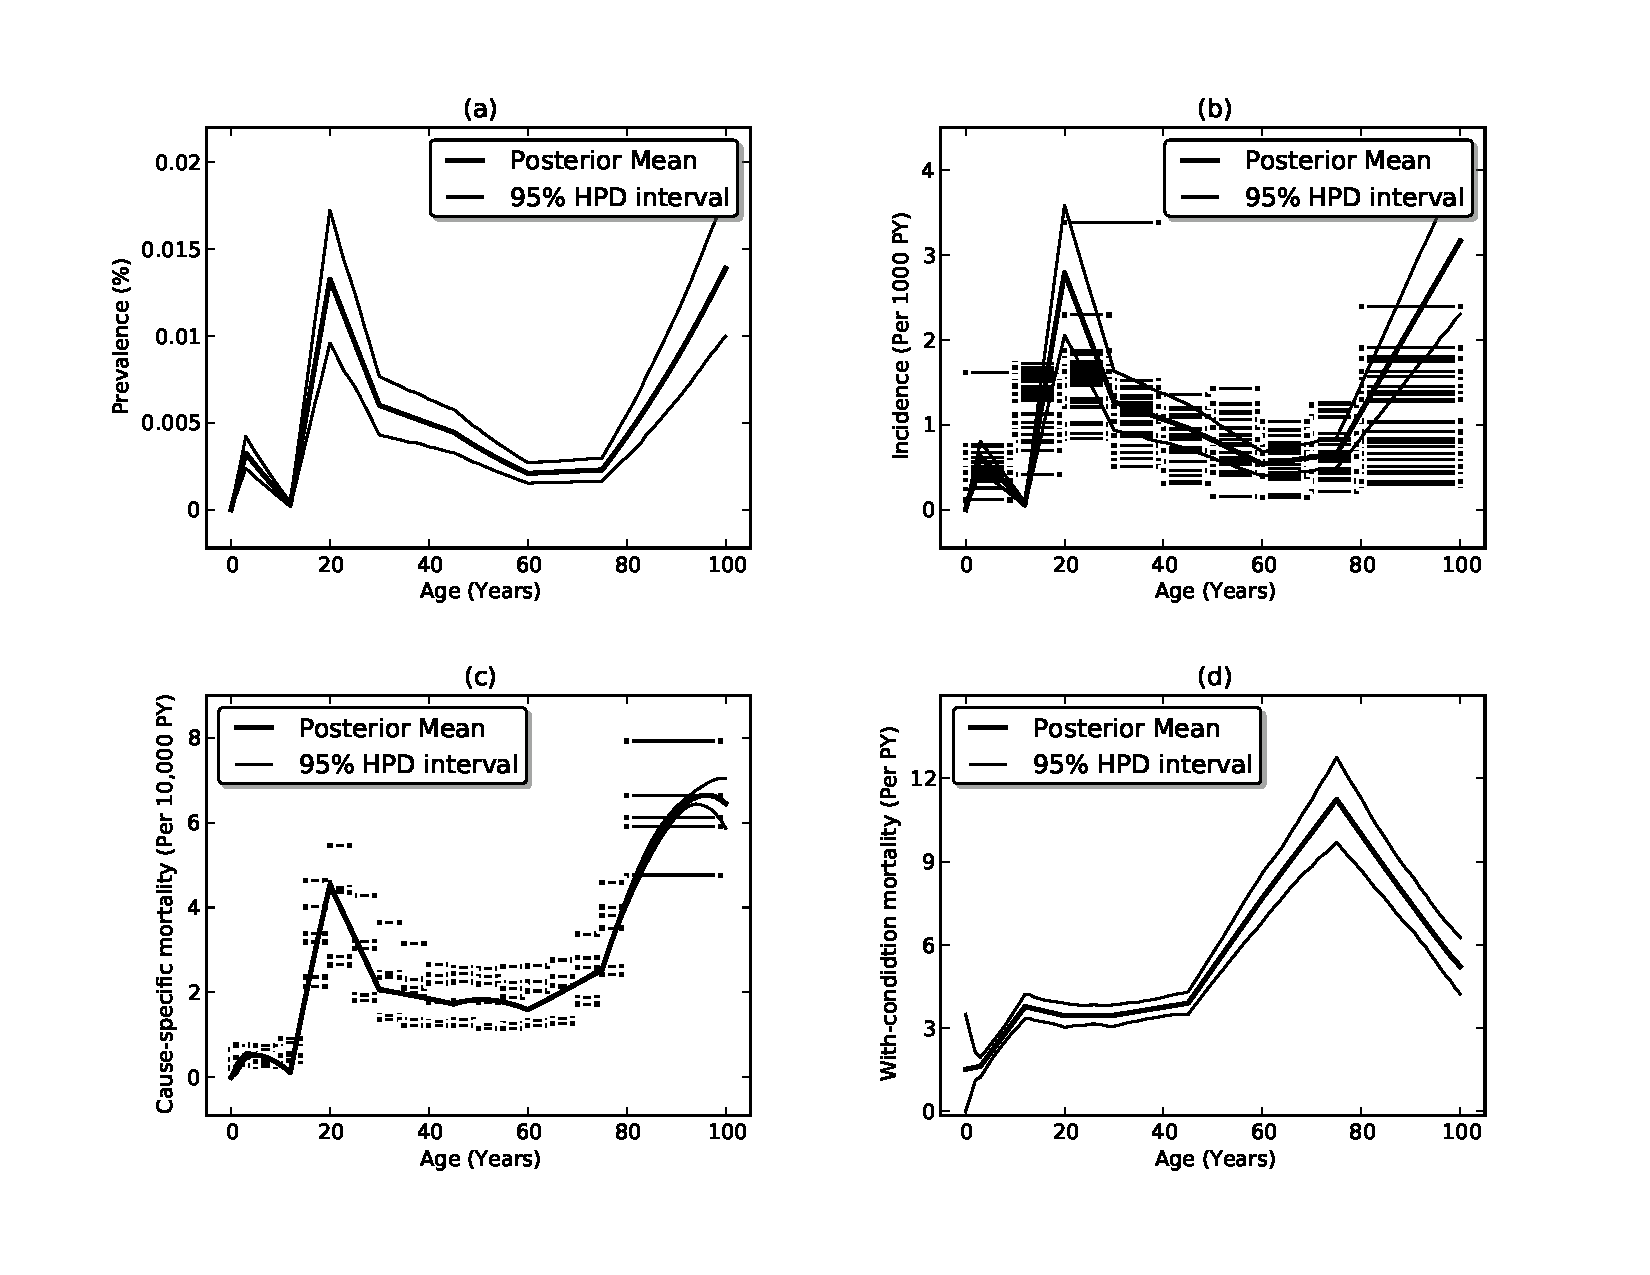
\includegraphics[width=\textwidth]{injuries-traffic_con_fit.pdf}
            \caption{Before being divided into long and short term outcomes, a compartmental model estimates the prevalence (a), incidence (b), cause-specific mortality (c) and with-condition mortality (d) for males in the United States of America in 2005.}
            \label{fig:app-injury traffic fit}
        \end{center}
    \end{figure}

As discussed, injuries have a wide range of outcomes.  Dividing incidence into short and long term outcomes avoids violating the assumption of a constant mortality hazard.  Once long term traffic injury incidence is extracted, it is further subdivided into the nature of the injury, such as fractures, burns, amputations or traumatic brain injury.  Figure \ref{fig:app-injury brain data} shows incidence data for moderate to severe traumatic brain injury warranting hospital admission or other health care in North America.

    \begin{figure}[h]
        \begin{center}
            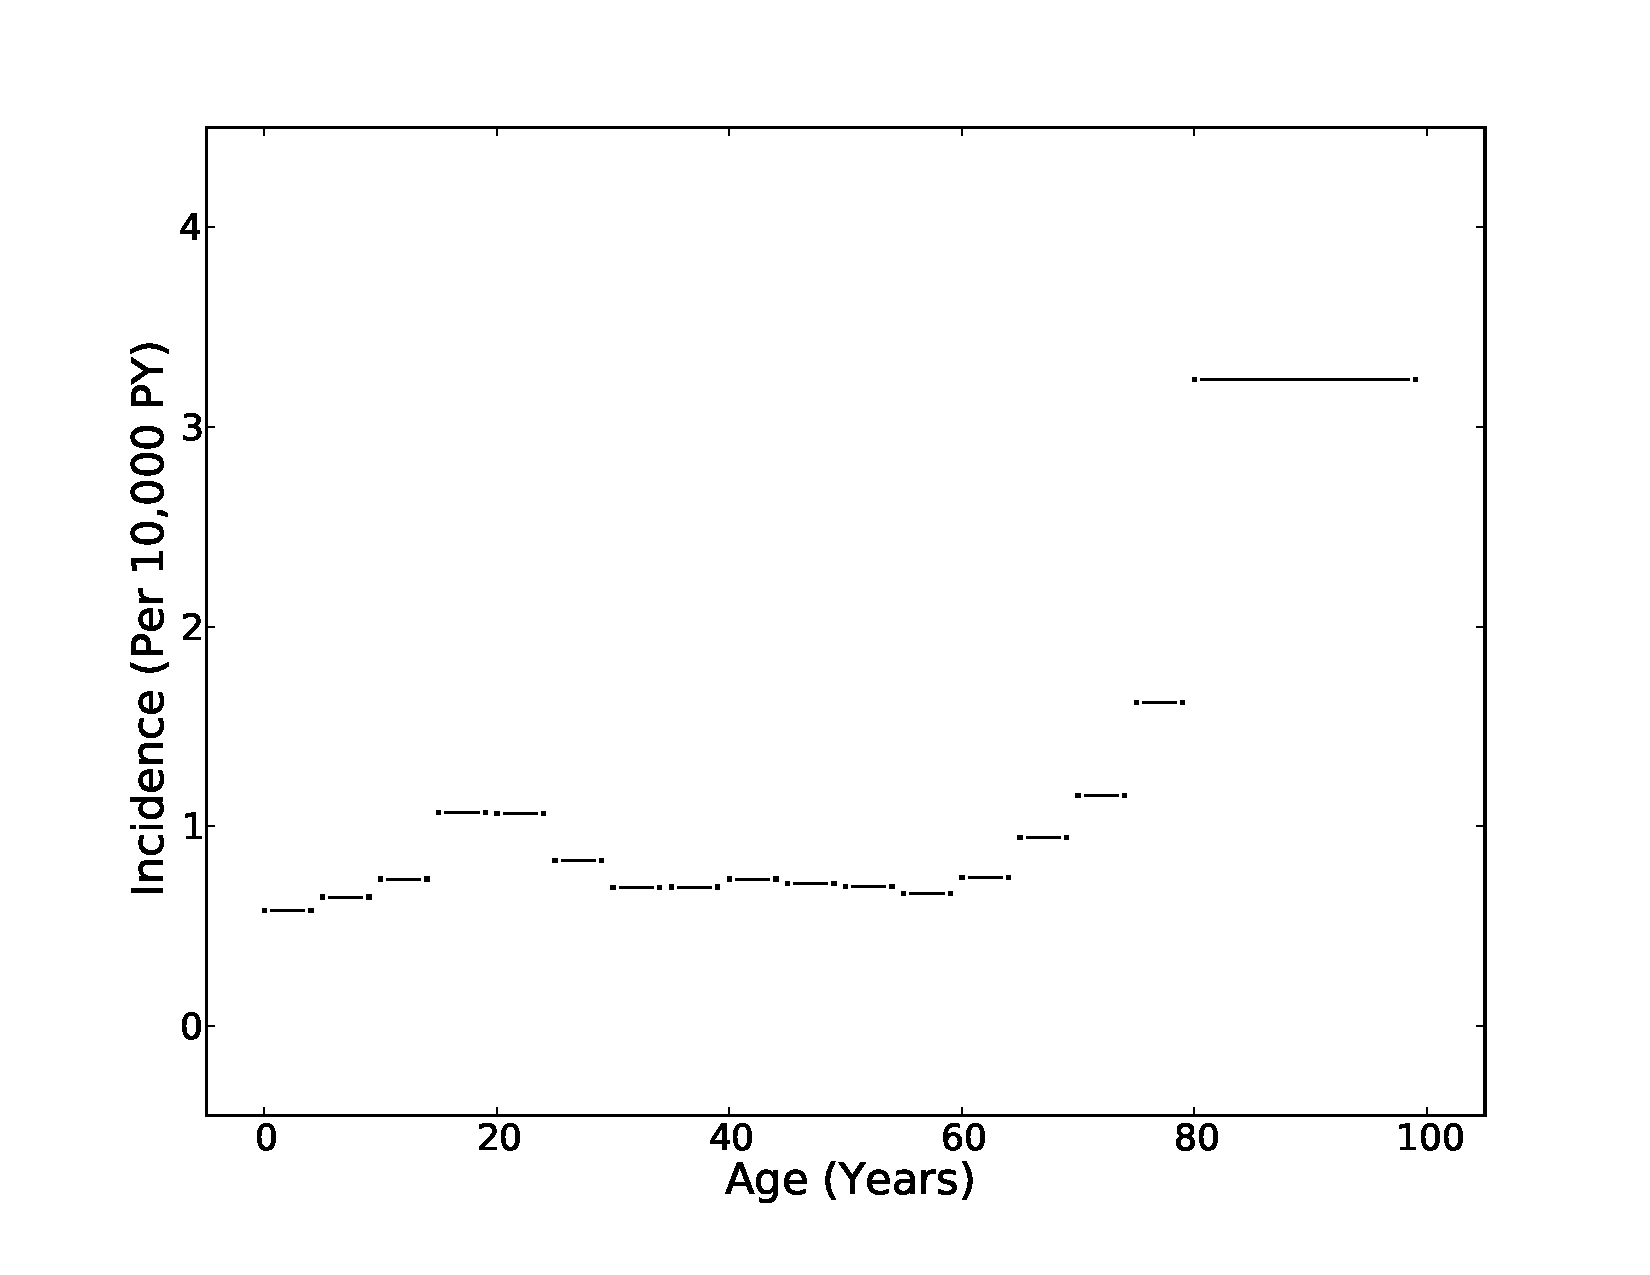
\includegraphics[width=\textwidth]{injury-brain_data.pdf}
            \caption{Long-term incidence data for moderate and severe traumatic brain injury in the region of North America, High Income.}
            \label{fig:app-injury brain data}
        \end{center}
    \end{figure}

From this, a compartmental model can estimate prevalence and incidence of moderate to severe traumatic brain injury caused by traffic injuries, as shown in Figure \ref{fig:app-injury brain fit}

    \begin{figure}[h]
        \begin{center}
            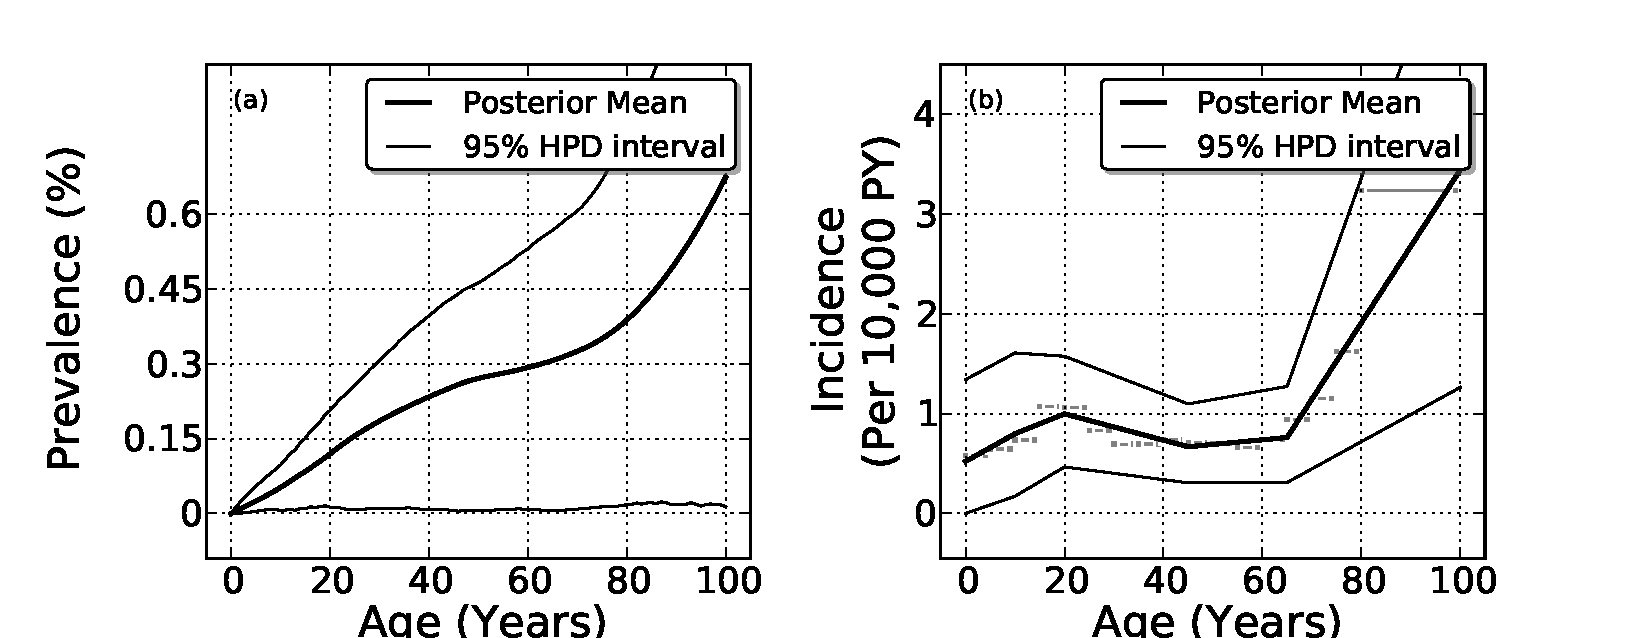
\includegraphics[width=\textwidth]{injuries-con_fit_p.pdf}
            \caption{The prevalence (a) and incidence (b) estimates for males in the United States of America in 2005 with moderate to severe traumatic brain injury caused by traffic injuries.}
            \label{fig:app-injury brain fit}
        \end{center}
    \end{figure}



